% CREATED BY DAVID FRISK, 2016

% IMPORT SETTINGS
\documentclass[12pt,a4paper,twoside,openright]{report}
% CREATED BY DAVID FRISK, 2016

% NOTE(Bjorn): Added packages.
\usepackage{verbatim}                   % For block comments
\usepackage{verbatimbox}
\usepackage{cite}
% BASIC SETTINGS
\usepackage{moreverb}                   % List settings
\usepackage{textcomp}                   % Fonts, symbols etc.
\usepackage{lmodern}                    % Latin modern font
\usepackage{helvet}                     % Enables font switching
\usepackage[T1]{fontenc}                % Output settings
\usepackage[english]{babel}             % Language settings
\usepackage[utf8]{inputenc}             % Input settings
\usepackage{amsmath}                    % Mathematical expressions
\usepackage{amssymb}                    % Mathematical symbols
\usepackage{graphicx}                   % Figures
\usepackage{wrapfig}					% Figures with text wrapping
\usepackage{subfig}                     % Enables subfigures
\numberwithin{equation}{chapter}        % Numbering order for equations
\numberwithin{figure}{chapter}          % Numbering order for figures
\numberwithin{table}{chapter}           % Numbering order for tables
\usepackage{listings}                   % Enables source code listings
\usepackage{chemfig}                    % Chemical structures
\usepackage[top=3cm, bottom=3cm,
            inner=3cm, outer=3cm]{geometry}     % Page margin lengths
\usepackage{eso-pic}                    % Create cover page background
\newcommand{\backgroundpic}[3]{
        \put(#1,#2){
        \parbox[b][\paperheight]{\paperwidth}{
        \centering
        \includegraphics[width=\paperwidth,height=\paperheight,
                         keepaspectratio]{#3}}}}
\usepackage{float}                      % Enables object position enforcement using[H]
\usepackage{parskip}                    % Enables vertical spaces correctly 



% Caption settings (aligned left with bold name)
\usepackage[labelfont=bf, textfont=normal,
                        justification=justified,
                        singlelinecheck=false]{caption}                 

                        
% Activate clickable links in table of contents         
\usepackage{hyperref}                                                           
\hypersetup{colorlinks, citecolor=black,
            filecolor=black, linkcolor=black,
            urlcolor=black}


% Define the number of section levels to be included in the t.o.c. 
% and numbered (3 is default)   
\setcounter{tocdepth}{5}                                                        
\setcounter{secnumdepth}{3}     


% Chapter title settings
\usepackage{titlesec}           
\titleformat{\chapter}[display]
  {\Huge\bfseries\filcenter}
  {{\fontsize{50pt}{1em}\vspace{-4.2ex}\selectfont \textnormal{\thechapter}}}{1ex}{}[]


% Header and footer settings (Select TWOSIDE or ONESIDE layout below)
\usepackage{fancyhdr}                                                           
\pagestyle{fancy}  
\renewcommand{\chaptermark}[1]{\markboth{\thechapter.\space#1}{}} 
\newcommand{\clash}{C$\lambda$aSH }


% Select one-sided (1) or two-sided (2) page numbering
\def\layout{2}  % Choose 1 for one-sided or 2 for two-sided layout
% Conditional expression based on the layout choice
\ifnum\layout=2 % Two-sided
    \fancyhf{}                                                                  
        \fancyhead[LE,RO]{\nouppercase{ \leftmark}}
        \fancyfoot[LE,RO]{\thepage}
        \fancypagestyle{plain}{                 % Redefine the plain page style
        \fancyhf{}
        \renewcommand{\headrulewidth}{0pt}              
        \fancyfoot[LE,RO]{\thepage}}    
\else                   % One-sided     
        \fancyhf{}                                      
        \fancyhead[C]{\nouppercase{ \leftmark}}
        \fancyfoot[C]{\thepage}
\fi


% Enable To-do notes
\usepackage[textsize=tiny]{todonotes} % Include the option "disable" to hide all notes
\setlength{\marginparwidth}{2.5cm} 


% Supress warning from Texmaker about headheight
\setlength{\headheight}{15pt}           


\begin{document} 

% COVER PAGE, TITLE PAGE AND IMPRINT PAGE
% Roman numbering (starting with i (one)) until first main chapter
\pagenumbering{roman}

%%%%%%%%%%%%%%%%%%%%%%%%%%%%%%%%%%%%%%%%%%%%%%%%%%%%%%%%%%
% NOTE(Bjorn):Global Variables for the frontmatter section.
%%%%%%%%%%%%%%%%%%%%%%%%%%%%%%%%%%%%%%%%%%%%%%%%%%%%%%%%%%
% An Informative Headline describing\\ the Content of the Report
\newcommand{\varHeadline}{Sphere Tracing GPU Attempt}
% A Subtitle that can be Very Much Longer if Necessary
\newcommand{\varSubtitle}{A Graphics Processing Unit Designed to Use Sphere 
	Tracing for Rendering}
% Department of Some Subject or Technology
\newcommand{\varDepartment}{Department of Computer Science and Engineering}
% Division of Division name
\newcommand{\varDivision}{Undergrad}
% Name of research group (if applicable)
\newcommand{\varResearchGroupName}{DATX02-17-12}
% NAME FAMILYNAME
\newcommand{\varNames}{André Perzon, Björn Strömberg, Chi Thong Luong,  \\
Elias Forsberg, Jesper Åberg, Jon Johnsson}

%zipwith
\makeatletter
% \zipwith{<coupler>}{<list1>}{<list2>}{<return macro>}
% \zipwith*{<coupler>}{<listcmd1>}{<listcmd2>}{<return macro>}
\protected\def\zipwith{%
  \begingroup
  \@ifstar{\def\cnta{1}\@zipwith}
    {\def\cnta{0}\@zipwith}%
}
\def\@zipwith#1#2#3#4{%
  \def\tempa##1##2{%
    \edef##2{%
      \ifnum\cnta=\@ne\else\expandafter\@firstoftwo\fi
      \unexpanded\expandafter{##1}%
    }%
  }%
  \tempa{#2}\tempb\tempa{#3}\tempa
  \def\cnta{0}\def#4{}%
  \foreach \x in \tempb{%
    \xdef\cnta{\the\numexpr\cnta+1}%
    \gdef\cntb{0}%
    \foreach \y in \tempa{%
      \xdef\cntb{\the\numexpr\cntb+1}%
      \ifnum\cntb=\cnta\relax
        \xdef#4{#4\ifx#4\empty\else,\fi\x#1\y}%
        \breakforeach
      \fi
    }%
  }%
  \endgroup
}
\makeatother

%scatter plot command
%usage: 
%  \scatterplot{x1,x2,x3...}{y1,y2,y3}{xscale}{yscale}{xlabel}{ylabel}{datafile}
%    where datafile is a file with a list of x y coordinates (one space 
%    separated pair on each line)
\newcommand{\scatterplot}[7]{
	\begin{tikzpicture}[only marks, y=.5cm]
		\draw[->,xshift=-5.0cm] (5.0,0) -- coordinate (x axis mid) (14,0);
		\draw[->,xshift=-5.0cm] (5.0,0) -- coordinate (y axis mid) (5.0,14);
		\zipwith{/}{0,1.6,3.2,4.8,6.4,8}{#1}\xlist
		\foreach \x/\xtext [evaluate=\x as \xeval using 2*\x] in \xlist
			\draw (\x cm,1pt) -- (\x cm,-6pt)
			node[anchor=north] {$\xtext$};
		\zipwith{/}{0,1.3,2.6,3.9,5.2,6.5}{#2}\ylist
		\foreach \y/\ytext in \ylist
			\draw (1pt,\y cm) -- (-3pt,\y cm) 
			node[anchor=east] {$\ytext$};
		\node[below=1cm] at (x axis mid) {#5};
		\node[anchor=south,left=1.5cm,rotate=90] at (y axis mid) {#6};
		
		\foreach \ys [evaluate=\ys as \ysc using 0.01*\ys] in {#4} {
			\foreach \xs [evaluate=\xs as \xsc using 0.1*\xs] in {#3} {	
				\draw plot[y=\ysc cm,x=\xsc cm,mark=*] file {#7};
			}
		}
	\end{tikzpicture}
}

% CREATED BY DAVID FRISK, 2016

% COVER PAGE
\begin{titlepage}
\newgeometry{top=3cm, bottom=3cm,
			left=2.25 cm, right=2.25cm}	% Temporarily change margins		
			
% Cover page background 
\AddToShipoutPicture*{\backgroundpic{-4}{56.7}{figure/auxiliary/frontpage_eng.pdf}}
\addtolength{\voffset}{2cm}

% Cover picture (replace with your own or delete)		
\begin{figure}[H]
\centering
\vspace{2cm}	% Adjust vertical spacing here
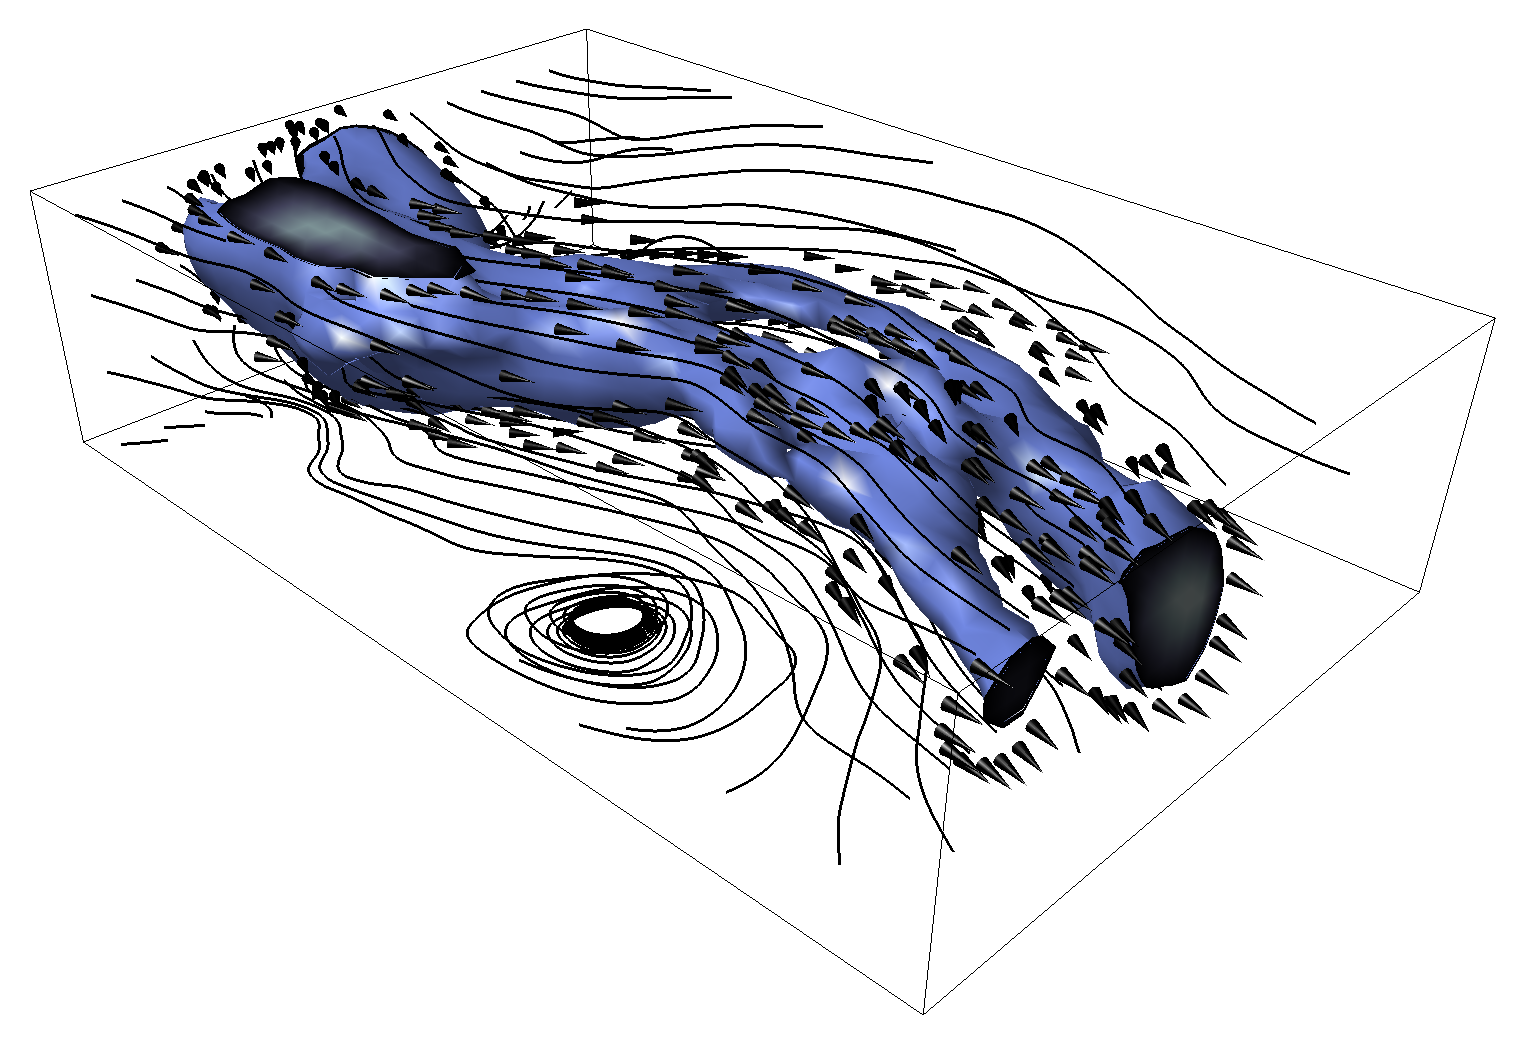
\includegraphics[width=0.9\linewidth]{figure/Wind.png}
\end{figure}

% Cover text
\mbox{}
\vfill
\renewcommand{\familydefault}{\sfdefault} \normalfont % Set cover page font
\textbf{{\Huge 	\varHeadline}} 	\\[0.5cm]
{\Large \varSubtitle}\\[0.5cm] Bachelor's thesis in Computer Science \setlength{\parskip}{1cm}

{\Large \varNames} \setlength{\parskip}{2.9cm}

\varDepartment \\
\textsc{Chalmers University of Technology} \\
Gothenburg, Sweden 2016

\renewcommand{\familydefault}{\rmdefault} \normalfont % Reset standard font
\end{titlepage}


% BACK OF COVER PAGE (BLANK PAGE)
\newpage
\restoregeometry
\thispagestyle{empty}
\mbox{}


% TITLE PAGE
\newpage
\thispagestyle{empty}
\begin{center}
	\textsc{\large Master's thesis 2016:NN}\\[4cm]		% Report number given by department 
	\textbf{\Large \varHeadline} \\[1cm]
	{\large \varSubtitle}\\[1cm]
	{\large \varNames}
	
	\vfill	
	% Logotype on titlepage	
	\begin{figure}[H]
	\centering
	% Remove the following line to remove the titlepage logotype
	
\includegraphics[width=0.2\pdfpagewidth]{figure/auxiliary/logo_eng.pdf} \\	
	\end{figure}	\vspace{5mm}	
	
	\varDepartment \\
	\emph{\varDivision}\\
	\varResearchGroupName\\
	\textsc{Chalmers University of Technology} \\
	Gothenburg, Sweden 2016 \\
\end{center}


% IMPRINT PAGE (BACK OF TITLE PAGE)
\newpage
\thispagestyle{plain}
\vspace*{4.5cm}
\varHeadline \\
\varSubtitle \\
\varNames \setlength{\parskip}{1cm}

\copyright ~ \varNames, 2016. \setlength{\parskip}{1cm}

Supervisor: Name, Company or Department\\
Examiner: Name, Department \setlength{\parskip}{1cm}

Master's Thesis 2016:NN\\	% Report number given by department 
\varDepartment \\
\varDivision \\
\varResearchGroupName\\
Chalmers University of Technology\\
SE-412 96 Gothenburg\\
Telephone +46 31 772 1000 \setlength{\parskip}{0.5cm}

\vfill
% Caption for cover page figure if used, possibly with reference to further information in the report
Cover: Wind visualization constructed in Matlab showing a surface of constant wind speed along with streamlines of the flow. \setlength{\parskip}{0.5cm}

Typeset in \LaTeX \\
Printed by [Name of printing company]\\
Gothenburg, Sweden 2016



% ABSTRACT
\newpage
\thispagestyle{plain}			% Supress header 
\setlength{\parskip}{0pt plus 1.0pt}

\section*{Abstract}
	
	Real-time rendering speed has always been a significant factor for 3D
	graphic cards. However, 3D graphic cards today are optimized and built for
	the polygon-based rendering. Therefore, Sphere Tracing rendering is slower
	in this hardware.  The aim of this thesis is to implement and design a
	basic GPU (Graphic proccesing unit) that could execute Sphere tracing.
	Subsequent to this, some optimizations were implemented in order to further
	assess the potential performance of the Sphere Tracing algorithm.
	
	This thesis documents the result of us examining the Sphere Tracing
	algorithm and designing a Graphics Processing Unit (GPU) to run it, using
	\clash, a functional hardware description language. In addition, possible
	future work are discussed.

	% KEYWORDS (MAXIMUM 10 WORDS)
	\vfill
	Keywords: sphere tracing, ray marching, ray tracing, GPU, real-time rendering.

\newpage
\thispagestyle{plain}

\section*{Sammanfattning}
	
	Denna uppsats dokumenterar resultaten kring en grafikenhet (GPU) som vi
	designat med avseende att köra en specifik rendreringsalgoritm kallad Sphere
	Tracing, en typ av Ray Tracing. GPUn är skriven i det funktionella
	hårdvarubeskrivande programmeringsspråket (FHDL) \clash.
	
	Hastigheten på realtidsrenderingen hos 3D grafikkort har alltid varit en
	viktig säljpunkt. Dock, när det kommer till Sphere Tracing rendrering jämfört
	med polygonbaserade rendreringsmetoder så har den förstnämda historiskt sett
	varit långsammare. Detta har lett till att man vidareutvecklat hårdvaran
	specifikt för att accelerera polygonrendrering vilket leder till frågan hur
	pass snabbt Sphere Tracing kan köras om liknande hårdvara skräddarsys för
	just den algoritmen. Avsikten med denna rapporten är att ge en idé om vilka
	prestandaökningar som finns att uppnå med ett alternativt realtidsrenderande
	3D grafikkort.
	
	% KEYWORDS (MAXIMUM 10 WORDS)
	\vfill
	Nyckelord: bollkoll, sphere tracing, ray marching, ray tracing, realtidsrendering.


\newpage
\thispagestyle{empty}
\mbox{}


% TABLE OF CONTENTS
\newpage
\tableofcontents

% TODO(Bjorn): Do we really want this?
%% OTHER FRONTMATTER
%% List of figures (add to table of contents)
%\cleardoublepage
%\addcontentsline{toc}{chapter}{\listfigurename} 
%\listoffigures
%% List of tables (add to table of contents)
%\cleardoublepage
%\addcontentsline{toc}{chapter}{\listtablename}  
%\listoftables

% START OF MAIN DOCUMENT
%\cleardoublepage
\newpage
\setcounter{page}{1}
\pagenumbering{arabic}
\setlength{\parskip}{0pt plus 1pt}

% INTRODUCTION
% CREATED BY DAVID FRISK, 2016
\chapter{Introduction} 

The algorithm in question that we designed a custom GPU for is called sphere
tracing.\cite{Hart1996} So called since it uses spheres to incrementally
advance a ray in 3D space. The method of advancing rays incrementally is called
ray marching and is a particular subset of ray tracing.\cite{Whitted1980} Ray
tracing, then, is a way of wholly or partially rendering the world through
rays, cast from the eye of the observer into the scene.  Sphere tracing has
been around since at least as early as the late eighties and ray tracing as
early as the sixties.\cite{Hart1989,Appel1968} Since ray tracing traditionally
has been a more computation-intensive method compared to
scanlining\cite{Wylie1967} and as such it has generally seen more use in movie
production rather than in real-time applications.\cite{ref_needed?} 

%TODO(bjorn): Nån som är bätre än mig på detta får gärna skriva om denna delen
%             nedanför. låter inte proffsigt alls.

The advent of the programmable shader brought back the discussion of real time
ray marching to the forefront. which is where we caught on to it.
\cite{JamieWong2016} It still favours poorly compared to other techniques which
natrually begged the question if it would be able to compete in real time if
only the hardware for it was there.

\section{Sphere tracing} 

\begin{minipage}{0.6\textwidth} 

	At the base of the algorithm are the signed distance functions.
	$$\text{SDF}:\mathbb{R}^{3}\mapsto\mathbb{R}$$ The "distance" is the distance
	between a point and the closest point on the implicit surface
	$\text{SDF}^{-1}(0)$. The "signed" part refers to the distance being negated
	when measured inside of the surface.  If we define a ray $$r(s) = \vec{d}
	\cdot s + \vec{o}$$ where $\vec{d}$ is the normalized direction of the ray
	and $\vec{o}$ the origin, then $$\text{SDF}\circ r(s) = 0$$ means that the
	ray intersects a surface at exactly the distance $s$ from its origin.

\end{minipage} 

\hfill
\begin{minipage}{0.3\textwidth}
	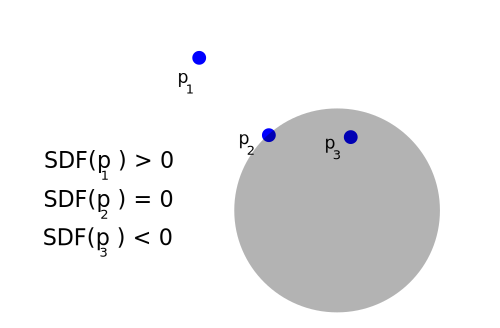
\includegraphics[width=\linewidth]{figure/SDF} 
\end{minipage}

\bigskip

Finding the surface can be done by iterating point by point from the origin
along the ray like below. $$p_{i+1} = p_i + \vec{d}\cdot \text{SDF}(p_i)$$ This
is repeated until $\text{SDF}(p_i) \leq \varepsilon$ for a given precision
limit $\varepsilon$. $\text{SDF}(p_i)$ is the furthest we can march the ray
while still be sure we don't overshoot any potential surfaces.  The direction
of the closest surface point is never known thus $\text{SDF}(p_i)$ can be
interpreted as a sphere bound, giving the algorithm its namesake. This ray
marching is then performed for each pixel of the screen reversely simulating
the light rays from a scene entering the lens of the onlooker.
	
	\subsection{Reflections and refractions}

	Once a point on a surface for a given pixel has been located new multiple
	rays can then be further marched to determine reflections, towards the
	scene's sources of light determening light and shadows, or through the object
	with an angle, simulating refractions. A lot of these depend on the surface
	normal which can be calculated by normalizing the aproximate gradient of
	$\text{SDF}(p)$. 

	\subsection{Textures}

	Texturizing could at least be done in two ways. The straightforward way would
	be to use the surface point coupled with an id-signature of the figure. After
	translating and re-scaling the point to the origin, it could then be directly
	looked up in a 1:1 3D texture as per its id. A more indirect but space-saving
	alternative could be to replace the last step with a sphere trace from the
	translated point along its surface normal\footnotemark out towards a simple
	wrapping geometry. The resulting surface coordinate could then along with the
	whole surface be transformed into a 2D flat plane mapping to a corresponding
	2D texture. The texture and enclosing geometry again being variable according
	to the id of the figure.

	\footnotetext{Or along the normal of the point.}

\section{Hardware implementation}


% PROBLEM DESCRIPTION
\chapter{Problem Description}

	The main problem is to identify the critical parts of the algorithm that
	prevents it from being a feasible alternative today, and to figure out a
	 hardware design that improves the performance of those parts. Following are the
	questions we worked to answer throughout the project.
	
	\begin{itemize}
		\item How does sphere tracing work?
		\item What language is best suited to describe the GPU?
		\item Are there ways we can improve the algorithm at a theoretical 
			level?
		\item How do we architect for parallelism and multiple cores?
		\item What mathematical functions are best implemented in hardware vs 
			software?
	\end{itemize}


% STATE OF THE ART / LITERATURE
\chapter{State of the Art}

	\section{ Real Time Graphics Rendering on Current Hardware } 

		Sphere tracing is currently being used to visualize complex data such
		as fractals \cite{granskog2017}, but there is no hardware designed to
		run it efficiently.  Today's top of the line consumer 3D graphics cards
		are made for real time rendering of polygons\cite{Houston2010}. They achieve good
		performance by executing rasterization and pixel color calculation in
		parallel between pixels. To make this efficient they use what is known
		as lockstepping, which means a group of calculation units that are
		always operating on the same instruction, but with differing input
		data. This enables all of the cooperating cores to use only a single
		instruction memory and bus. This reduces the area usage of the design,
		making it possible to add more cores per chip and thus achieve greater
		performance. Pixels rendered by polygon based methods can usually be
		queued for calculation in such a way that pixels belonging to the same
		object in the scene can be grouped for computation. The drawback of
		lockstepped cores only being able to work on the same instruction at a
		time is thus greatly reduced.
		
		Using this hardware for Sphere Tracing, as is currently being done,
		increases the overhead caused by this lockstepped design significantly.
		Order of pixel rendering in a polygon renderer is done by object and
		then by constituent polygons. Pixels can not be grouped by what object
		in the scene they belong to as easily in a Sphere Tracer, because Sphere
		Tracers do not have polygons and pixel order is usually based on the
		output image pixel order. Even if more grouping was introduced to a
		Sphere Tracer, the pixels in these groups differ much more in their
		instruction execution path, since the algorithm is more iterative and
		often varies greatly in number of steps until completion.

		\section{ Hobbyists and Academia }
\cite{
		Despite this, computer art hobbyists are using Sphere Tracing to produce
		some quite stunning real time visuals on consumer PC's. They showcase 
		the possibilities of the algorithm by reducing scene complexity and 
		instead rendering using techniques that are commonly found in non 
		real time Ray Tracers. Examples of such are true reflections and 
		refractions, spacial repetition, object morphing and 3D fractals. 
		For some examples of this check out ???  \cite{InigoQuilez}.
		Inspired by research papers such as John C. Hart's 
		1996 paper\cite{Hart1996}, their success encouraged hobbyist to do 
		academic research of their own, which led to new papers being written. A 
		good example of this is the 2014 paper "Enhanced Sphere 
		Tracing"\cite{Korndorfer2014}.

		\section{ Industry }		
		% Kanske helt orelevant ?
		There are as of today no big commercial applications using Sphere Tracing
		that we know of, but Ray Tracing algorithms have long been in use in
		multiple computer graphics domains. For instance in film making
		\cite{Christensen2006}, where a comparatively large amount of time to
		render a scene can be acceptable but the demand for realism is higher
		than in real time graphics. An example of this would be the Ray Tracing
		engine RenderMan developed by Disney Pixar which is used in their movies
		\cite{Christensen2006}.
	
	\section{ Hardware Design Methods } 
	
		The design of Integrated Circuits in the hardware industry has since the early
		'90s primarily been done in hardware description languages (HDL)
		\cite{Chen2012}, where one describes the operation of a chip in a style similar to regular imperative programming languages. This descriptive
		code can then be compiled into a list of components and connections
		that constitutes the blueprint for that specific circuit. The most
		prevalent of these languages are VHDL and Verilog\cite{TODO}. While
		being great help to designers, compared to more manual design, these
		languages can be quite cumbersome to work with. They are verbose and 
		require a fair amount of boilerplate code. This makes it more difficult
		to understand, follow, and also write code that performs complex tasks, 
		since it can be more difficult to see the greater patterns in 
		interconnecting code\cite{TODO}.
		
		This has resulted in Functional HDLs (FHDL): ``Functional hardware
		description languages are a class of hardware description languages
		that emphasize on the ability to express higher level structural
		properties, such a parameterization and regularity. Due to such
		features as higher-order functions and polymorphism, parameterization
		in functional hardware description languages is more natural than the
		parameterization support found in the more traditional hardware
		description languages, like VHDL and Verilog'' \cite{Baaij2009}
		
		HDLs have been around since the late '70s \cite{Chen2012},
		but in recent times they have become more mature\cite{TODO}. There are in
		particular two FHDLs, \emph{Lava} and \clash \cite{Baaij2009},
		Bjesse1998}, that are implemented in Haskell. This allows the same
		interactive type checking and high-level simulation of the program that
		normal Haskell programs enjoy. This means that instead of simulating
		the underlying circuit directly which is more time consuming, the

		design can be tested repeatedly at a faster pace, allowing faster
		development. This high level simulation can also be done in an
		interpreter enabling easy and rapid testing of code. These are called
		read-eval-print-loop interpreters.



% THEORY
% CREATED BY DAVID FRISK, 2016
\chapter{Sphere Tracing} \label{spheretracing}

	% TODO(bjorn):
	% fixa bild r krockar

	The graphics rendering algorithm in question that we designed a custom GPU
	for is called Sphere Tracing\cite{Hart1996}. The name comes from the
	technique where it uses spheres to incrementally advance a ray in 3D space.
	The method of advancing rays incrementally is called Ray Marching and is a
	particular subset of ray tracing\cite{Whitted1980}. Ray Tracing, then, is a
	way of wholly or partially render the world through rays, cast from the eye
	of the observer into the scene. Sphere Tracing has been around since at least
	as early as the late eighties\cite{Hart1989} and Ray Tracing as early as the
	sixties\cite{Appel1968}. Ray Tracing has traditionally been a more
	computationally intensive method compared to polygon
	rendering\cite{Wylie1967} and thus it has generally seen more use in movie

	production rather than in real-time applications.\cite{ref_needed?} 

	The advent of per pixel programmable hardware in graphics cards made it 
	possible to implement real time graphics rendering based on ray	marching, 
	albeit only using relatively simple geometry. This raises the question of 
	whether this rendering method could be competitive for real time graphics 
	if hardware that was specifically designed for it was available.

	In this chapter we walk through the Sphere Tracing algorithm in detail with
	both definitions and examples. The explanation is based on the the very
	succint explanation in \cite{Korndorfer2014} where they also expand upon the
	original algorithm. For a more in-depth description we refer to Harts
	``\emph{Sphere tracing: a geometric method for the antialiased ray tracing
	of implicit surfaces}``\cite{Hart1996} as the de-facto explanation.


	\section{Sphere Tracing} 

		\begin{wrapfigure}{r}{0.48\textwidth}
			\begin{flushright}
				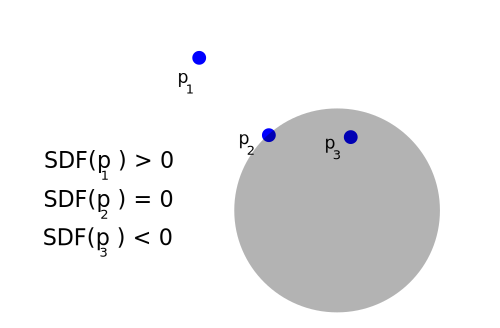
\includegraphics[width=0.9\linewidth]{figure/SDF} 
			\end{flushright}
			\caption{ Signed Distance Function of a sphere, sampled at three points}
			\vspace{40pt}
		\end{wrapfigure}

		The sphere tracing algorithm is based on the concept of Signed Distance
		Functions (SDF).  $$\text{SDF}:\mathbb{R}^{3}\mapsto\mathbb{R}$$ The
		``distance`` is the distance between a point and the closest point on the
		implicit surface $\text{SDF}^{-1}(0)$. The ``signed`` part refers to the
		distance being negated when measured on the other side of the surface. 

		A common example would be the SDF of a sphere centered at the origin with a
		radius of one. $$\text{SDF}(\vec{v}) = |\vec{v}| - 1$$ We can here see that
		a point $\vec{v}$ exactly on the surface would evaluate to $1 - 1 = 0$
		where any point outside of the sphere being positive and any point inside
		the sphere being negative. In this case the absolute of the result would
		also describe the smallest distance to the surface but this is not a hard
		constriction for the algorithm to work.

		\vspace{40pt}
		\begin{wrapfigure}{r}{0.48\textwidth}
			\begin{flushright}
				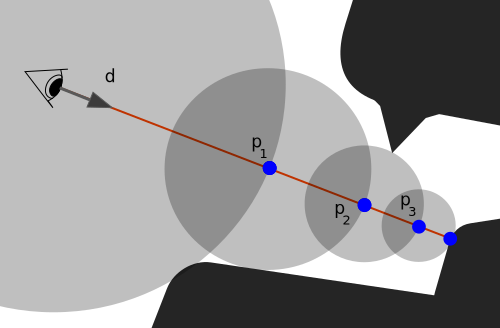
\includegraphics[width=0.9\linewidth]{figure/SDF2} 
			\end{flushright}
			\caption{A single ray marching according to Sphere Tracing}
			\vspace{40pt}
		\end{wrapfigure}

		If we define a ray $$r(s) = \vec{d} \cdot s + \vec{o}$$
		where $\vec{d}$ is the direction of the ray and $\vec{o}$ the origin, then
		$$\text{SDF}\circ r(s) = 0$$ means that the ray intersects a surface at
		exactly the distance $s$ from its origin. \emph{Sampling every SDF in a
		given scene and returning the smallest value yields a function known as a
		distance field.}

		\bigskip \noindent Finding the surface can be done by iterating point by
		point from the origin along the ray like below: $$p_{i+1} = p_i +
		\vec{d}\cdot \text{SDF}(p_i)$$ This is repeated until $\text{SDF}(p_i) \leq
		\varepsilon$ for a given precision limit $\varepsilon$. $\text{SDF}(p_i)$
		is the furthest possible march distance the ray can march while still being
		sure not too overshoot any potential surfaces. The direction of the closest
		surface point is never known, thus $\text{SDF}(p_i)$ can be interpreted as
		a spherical bound, giving the algorithm it's name. This Ray Marching is
		then performed for each pixel of the screen, reversely simulating the light
		rays entering the lens of an eye or camera.

			\subsection{Reflections, refractions and shading}

				Once a point on a surface for a given pixel has been located
				reflections, light, shadows and refractions needs to be calculated. A
				lot of these depend on the surface normal which can be approximated by
				the partial derivatives around the surface point for some small delta
				$\delta$, i.e taking the gradient and then normalizing it.

				$$\vec{g} = \vec{x}\cdot\frac{\text{SDF}(x+\delta, y, z)}{\delta} +
				\vec{y}\cdot\frac{\text{SDF}(x, y+\delta, z)}{\delta} +
				\vec{z}\cdot\frac{\text{SDF}(x, y, z+\delta)}{\delta} $$

				$$\vec{n} = \frac{\vec{g}}{|\vec{g}|} $$

				A simple way to lightset the scene could for an example be to use Phong
				Lightning\cite{Phong}. But from here on out any number of algorithms
				can be used in combination to determine the final color. Shadows can be
				determined by further Sphere Tracing out towards the sources of light
				to check for obstructions. Same for reflections and refractions where
				further marching in proportionate angles to the angle of incidence can
				determine what objects add to surface.


% METHODS
\chapter{Implementation}

	In order to achieve the goals set in this project, two separate pieces of 
	software and one piece of hardware were written. The software programs are 
	two different implementations of a reference shader. The first of these was 
	written in GLSL for traditional graphics hardware (in our case it was 
	tested on a GeForce GTX 1060M), and the second is written in an assembly 
	language we designed for the Sphere Tracing processor. Both of these 
	shaders are described in section \ref{implshader}. The hardware is 
	comprised of a multi-core programmable parallel processing unit designed 
	for the Sphere Tracing algorithm, detailed in section \ref{implproc}. In 
	addition to these, a simple assembler was written for the assembly language
	used for the GPU.

	\section{Reference Shader} \label{implshader}

		The core of the Sphere Tracer is a simple while-loop. It calculates
		distance to the closest object in the scene by sampling the distance
		field and comparing its value at the current location to a predefined
		epsilon. If the value of the distance field is smaller, the ray has hit
		an object; the corresponding pixel's color is calculated and the loop
		is terminated, unless the material of the object in question is defined
		as being reflective.

		\subsection{GLSL Based}

			The shader which is made to run on conventional graphics hardware
			was made in the high-level shading language GLSL (short for OpenGL
			Shading Language). It runs the program for each pixel the shader is
			rendered on, using the screen-coordinates as input.

			Beyond the actual sphere tracing loop the direction of the ray is
			calculated using a camera direction vector and offsetting it by the
			current pixel's screen coordinates, placed orthogonally along the
			vector.  The distance of this placement defines the field of view
			of the camera. This needs to be done for each pixel being rendered.

			The final color of a pixel is based on the material ID assigned to
			the first object that the ray intersects. The color can then be
			either calculated by a material formula or be derived from a
			texture lookup. True 3D materials can be done by texturing but this
			generally needs a large data set and thus a formula is mostly
			preferred where three dimensional materials are employed. 2D
			texturing can be done by projecting points from a flat image onto a
			simple geometric shape  which is more or less enveloping the object
			in question. This is called texture-mapping and commonly uses
			simple shapes like planes, cubes, spheres and cylinders. 

			%FLOWCHART

		\subsection{Orthogonal culling}

			The most demanding parts of sphere tracing are that the distance to
			a lot of objects has to be calculated once for every march step.
			The number of steps taken depends on the scene but they can reach
			over a hundred. One way to increase the performance is to reduce
			the number of objects that the distance has to be calculated to,
			without reducing the actual number of objects in the scene. To do
			this the GPU needs to know which object a ray can't possibly hit,
			traditionally the CPU will tell the GPU which objects are in the
			field of view (Frustum culling) but we can't do that because of
			GLSL limitations. Even if we could use frustum culling it would
			probably not be enough, each ray should only care for the objects
			that it might hit, not all objects in the field of view.  An
			implementation of a method we call Orthogonal Culling was
			implemented.

			Orthogonal projection works by going through all the objects in the 
			scene for ray and calculating wheather the ray can hit the object
			or not. 

			To calculate whether the ray will hit a sphere or not orthogonal
			projection can be used. By projecting the center of the sphere onto
			the directional line of the ray, its closest point to the line is
			known.  Then the distance between the line and the sphere can be
			calculated using the radius, if the distance is less than zero the
			sphere will be hit by the ray. If the distance is larger than zero
			the ray can't possibly hit that sphere. This way the number of
			objects that the distance has to be calculated to is decreased.

		\subsection{Bounding spheres}
			
			Another way decrease the number of distance calculations that has
			to be performed in each march step is to enclose several objects in
			a march sphere. When the distance field is evaluated only the
			bounding sphere will be considered and none of the objects enclsed
			by it. If the bounding sphere is hit by the ray, it will be removed
			and all the contained objects will be introduced to the distance
			field. 

			In practice this was made by calculating the centrum of the
			objects, by adding together their position vectors and scale by the
			inverse of the number of objects, this point is the position of the
			bounding sphere. The radius of the sphere is simply the distance to
			the object that is the farthest from the center of the sphere plus
			it's "max radius", that is, for a cube with a side of length 2, the
			square root of 3. The way our bounding spheres was set up had some
			flaws, such as if huge objects are placed near origin of the
			bounding sphere it will only be partially rendered.

			%picture of example bounding sphere

		\subsection{GPU Assembler Based}

			In the assembler version that runs on our own hardware there is
			initially a single thread. This thread will create one new thread
			for each pixel on the screen, and this thread will calculate what 
			color the pixel should have and then terminate. This differs from 
			the shader version that simply runs the GLSL-code for each pixel
			in parallell at the graphics cards many cores.

	\section{Processor Unit} \label{implproc}

		The properties of the ray marching algorithm as described in chapter
		\ref{spheretracing} led to the decision of designing a GPU architecture
		that does not utilize multi-ALU SIMD with lockstepping to the same
		extent as traditional graphics processors. Instead, a solution with
		slightly simpler independent cores was decided upon. This is similar to
		reasoning employed by \cite{Woop2005} for a Ray Tracing hardware
		design.

		The hardware described in this section was written in \clash. \clash is
		based on the functional programming language Haskell and is therefore a
		functional hardware description language, or FHDL. One thing that
		\clash offered was the command-line repl that allowed us to quickly
		write and test new modules on a higher conceptual level rather than
		simulating the Verilog code on a bit level.

		\subsection{Architecture}

			The GPU is designed to be able to handle a form of threading
			natively, where all computations are performed by a thread running
			on some hardware core. A thread in this context is very
			light-weight: only an instruction pointer along with some mutable
			registers are stored.

			All threads that are not running are placed in a storage structure
			that is globally accessable to all cores, and threads are then
			dispatched to cores as the cores become available for execution.
			The cores are also able to spawn new threads by sending their data
			to the global storage, or terminate threads either by simply
			dropping them or by sending them to the frame buffer, where some of
			the registers will be used to determine the color of some pixel on
			the screen.

			Each core consists of instruction and data memories, some control 
			logic for execution order and a DFU. The data and instruction 
			memories are immutable and mirrored across all cores in their 
			entirety. The control logic is responsible for feeding the DFU with
			instructions and data, as well as updating the thread registers 
			when a new thread is attached, sending thread registers to the 
			global thread storage when new threads are spawned and and 
			requesting a new thread whenever the previously executing one 
			terminates.
			
			The DFU contains a stack which all arithmetic instructions operate
			on, as well as an ALU for carrying out calculations. It also keeps
			track of all the thread registers and updates them when such
			instructions are issued. The DFU contains very little extra control
			logic and is only able to receive and execute instructions, it does
			not keep track of any instruction pointers or when threads are
			attached or dropped, this is instead handled by the core control
			logic.

		\subsection{Instruction Set}

			A representation for distance functions was also designed. It is
			implemented as a reverse polish notation inspired stack based 
			instruction set.

			There are a total of four instruction types with different
			instruction encodings, their layout in memory is shown in figure
			\ref{encodingfig}, and the type of instructions are:

			\begin{description}
				\item[C-type] instructions are for control flow, that is, 
					instructions that affect the global queue or frame buffer or
					terminate the current thread. C-type instructions can be 
					conditionally executed, based on the condition encoded in
					the two highest bits in the opcode. 

				\item[D-type] instructions, which encode arithmetic- and vector
					instructions on the stack. These operate only on the
					internal stack in the core and not on any of the other
					registers. They can take up to six arguments and return up
					to three return values. D-type instructions can be split up
					in chunks using the \texttt{next} instruction, where the
					last computed result will be accumulated using the minimum
					automatically by the core.  This is useful for encoding
					distance functions.

				\item[V-type] instructions deal with memory accesses. The
					\texttt{p} bit encodes whether this access is for pack
					(mutable) or read-only memory.

				\item[R-type] instructions load wide immediate values into the
					DFU. They are currently only used for assigning distance
					function IDs.
			\end{description}

		\subsection{Execution Model}

			The processor contains a global storage structure that is shared
			among all cores, onto which all threads that are ready for
			execution wait until a core is ready to start executing them.

			\begin{figure}[H]
				\centering
				\caption{ XQBGPPPU Data flow diagram }
				\includegraphics[width=0.75\linewidth]{figure/dots/GPU-schematic.pdf} 
				\vspace{-4pt}
			\end{figure}
	
			Each shader thread has 16 mutable registers that are automatically
			loaded into the core when execution starts. These registers are
			also saved when execution pauses and they are also copied whenever
			a thread spawns a new child. The instruction \texttt{setval} can be
			used to change the value of a register, and the instruction
			\texttt{pack} reads the value of a register.

			All calculations are performed with intermediate values stored on a
			stack, with the ability to move any values between the stack and
			any of the registers using the \texttt{setval} and \texttt{pack}
			instructions.

			There are three main instructions for control flow: \texttt{pushq},
			\texttt{pushf}, and \texttt{drop}. Threads can spawn new threads at
			any time using the instruction \texttt{pushq}: this will cause the
			core to make a copy of all of the registers and push it onto the
			global queue, where another (or the same) core may later access
			them and start executing from the instruction pointer register
			(\texttt{r0}).

			Threads can also terminate execution in two ways. Executing the
			instruction \texttt{drop} will terminate the thread and discard all
			registers. Executing \texttt{pushf} will terminate the thread and
			discard all values except the pixel pointer (\texttt{r1}) and color
			register (\texttt{r2}), which will be sent to the frame buffer in
			order to be displayed on the screen.

			This set of instructions for control flow might initially seem to
			be neither useful nor easy to implement but they are powerful
			enough to implement for all branching that is needed in our ray
			marchers efficiently while being restrictive enough to make
			instruction memory accesses very predictable.

			In addition to this, each core can accelerate finding the minimum 
			distance for a set of distance functions using a built-in 
			accumulator, together with the instructions \texttt{next} and 
			\texttt{accum}. Because of this, distance functions can be written
			without any regard for how the shader that called them works, and
			this very common operation is automated, reducing the size of each
			distance function slightly.

		\subsection{Square Roots}

			Calculating distances is an integral part of the algorithm, so a
			good square root implementation was considered important for
			achieving good performance. Several different approaches for this
			were considered.

			Firstly, using an iterative method like Goldschmidt's or the
			babylonian method was considered. These require an initial starting
			value, which is usually generated using a look-up table. We tested
			a different and very fast method for generating an initial rough
			guess of the square root of any number without the need for a
			look-up table. A 16-bit version of this circuit is shown in figure
			\ref{orsqrt}, and an improved but slightly more expensive version
			is showed in figure \ref{orsqrt2}.  The basic working principle is
			based on the fact that the square root of a number har roughly half
			as many digits as the original number. In the version with slightly
			improved accuracy the placement of the extra wires is based on the
			bit pattern of $\sqrt{2}$.

			\begin{figure}
				\centering
				\caption{A simple square root approximator}
				\label{orsqrt}
				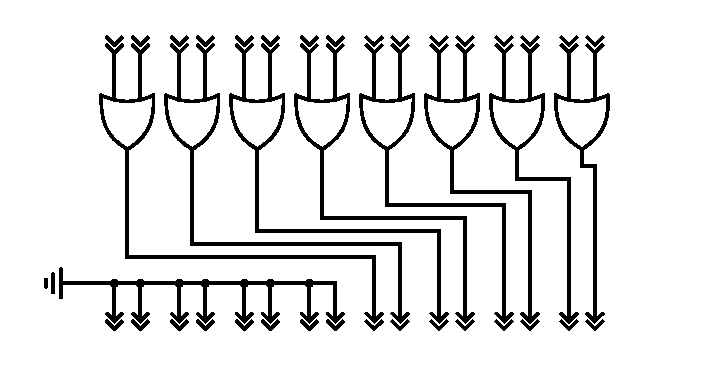
\includegraphics[width=0.75\linewidth]{figure/pdf/simpleOr.pdf} 
			\end{figure}

			\begin{figure}
				\centering
				\caption{Simple square root approximator with minor improvement}
				\label{orsqrt2}
				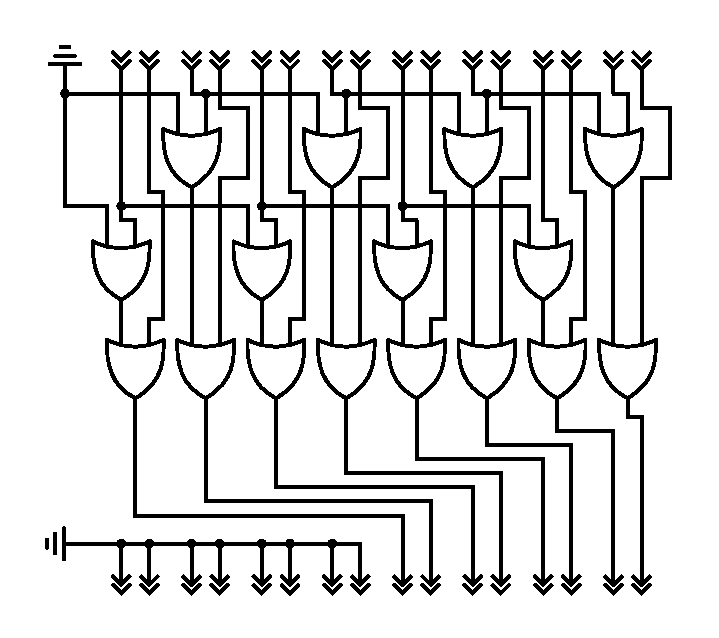
\includegraphics[width=0.75\linewidth]{figure/pdf/sqrt2Or.pdf} 
			\end{figure}

			In order to improve the accuracy of this method another design was
			considered in which the input was both rounded up and down to
			values where the simple square root approximator was very accurate
			and the result was then linearly interpolated between these roots.
			This linear interpolation requires only a multiplication and a
			couple of additions, but choosing upper and lower seed values is a
			more complex problem. Choosing the two geometrically closest powers
			of two was tested because the or-gate square root circuit is very
			accurate for powers of two, but this is not the only possible
			choice.

			\begin{table}
				\centering
				\caption{A \texttt{C} implementation of the shifting nth root 
					algorithm}
				\label{sqrtc}
				\begin{tabular}{c}
				\begin{lstlisting}
int isqrt(int num) {
    int res = 0;
    int bit = 1 << 30;

    while(bit != 0) {
        if(num >= res + bit) {
            num -= res + bit;
            res = (res >> 1) + bit;
        } else res >>= 1;
        bit >>= 2;
    }
    return res;
}
				\end{lstlisting}
				\end{tabular}
			\end{table}

			\begin{table}
				\centering
				\caption{A \texttt{C} implementation of the shifting nth root 
					algorithm}
				\label{sqrtcopt}
				\begin{tabular}{c}
				\begin{lstlisting}
int isqrt(int num) {
    int res = 0;
    int bit = 1 << 30;

    while(bit != 0) {
    	int tmp = num - (res | bit);
    	res >>= 1;
        if(tmp >= 0) {
            num = tmp;
            res |= bit;
        }
        bit >>= 2;
    }
    return res;
}
				\end{lstlisting}
				\end{tabular}
			\end{table}

			Another algorithm for calculating square roots is the
			\emph{Shifting nth root algorithm}, also known as \emph{Dijkstras
			square root algorithm}, which calculates the square root one digit
			at a time. A \texttt{c} implementation of this algorithm is shown
			in figure \ref{sqrtc}. Initially, this algorithm does not seem like
			a good canditate for a high performance hardware implementation,
			but several important optimizations are possible when unrolling it
			combinatorially. Most of the additions can be reduced to bitwise
			logic operations already when computing it in software, as shown in
			figure \ref{sqrtcopt}. In a combinatorial hardware implementation,
			these bitwise operations can be removed entirely by simply moving
			wires around, yeilding a logic cost of 0. The only remaining
			operations is therefore the subtraction on line 6, and the
			conditional assignments of \texttt{num} and \texttt{res} on lines 9
			and 10. The cost of the subtraction can be significantly reduced
			because \texttt{res} approximates the result one bit every step,
			meaning most bits are zeroed at any given iteration. On average,
			only 25\% of this subtraction is needed. This turned out to result
			in a design very similar to the PARSQRT implementation by
			\cite{japaneseSQRT}.


% RESULTS
\chapter{Results}

	In this chapter the results of GPU design choices and algorithmic
	optimizations and their effects are reviewed.

	\section{Software Shader Performance}

		The shader performed as expected, a conventional graphics card is
		capable of rendering scenes with low scene complexity in real-time
		using sphere tracing.

		Scenes can easily be made to look a lot more complex than they
		are, for example, by using mod fields, when the modulo
		operation is used on an object it creates a field with multiple copies
		of the original object next to each other, or fractals. The hardware
		(Geforce GTX 1060M) that the shader was tested on was able to render 20
		reflective spheres in real time in fullHD using our performance
		enhancing algorithm.
 
	\section{GPU}
	
		The GPU has been tested by simulating it and running a program on the simulation 
		that renders a sphere using Sphere Tracing. It spawns threads
		progressively to fill the screen data buffer with pixels. The execution
		of our test programs ran exactly as intended, with any number of
		simulated cores. The design has also been put through a synthesizing
		tool for FPGAs, which creates a net list of the components and
		connections that constitute the GPU. This also works as intended
		without any unexpected problems, but the actual operation of the GPU on
		an FPGA has not yet been verified.
	
	\section{Square roots}
		
		The accuracy of the different square root approximation and calculation
		methods are shown in figures \ref{sres1}, \ref{sres2}, \ref{sres3},
		\ref{sres4}, \ref{sres5}, and \ref{sres6}. The shifting nth root
		algorithm is used as a reference in all figures because it is always
		bit-accurate for integer square roots.

		\begin{figure}[H]
			\centering
			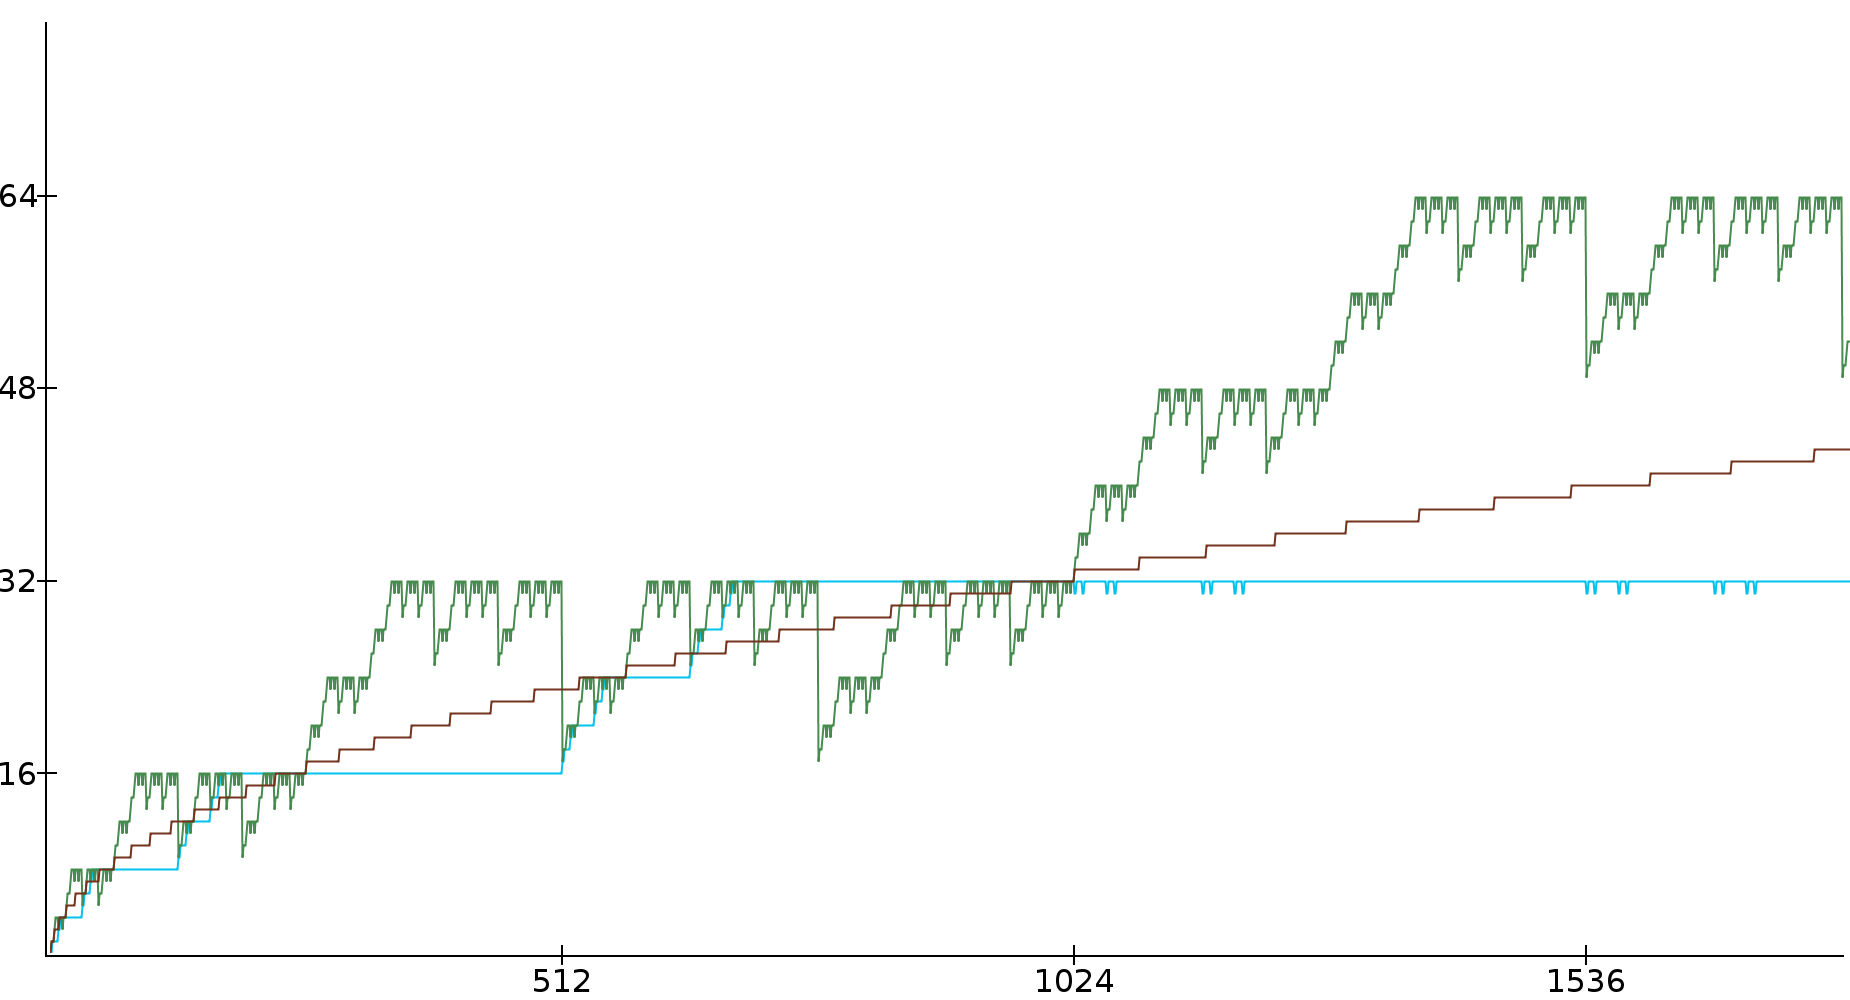
\includegraphics[width=0.75\linewidth]{figure/value12x.png} 
			\caption{Value from the simple square root approximator (green),
				the improved version (blue), and the shifting nth root 
				algorithm (red). In these graphs, they all operate on integers. 
				The shifting nth root is exact for integer square roots.}
			\label{sres1}
		\end{figure}

		\begin{figure}[H]
			\centering
			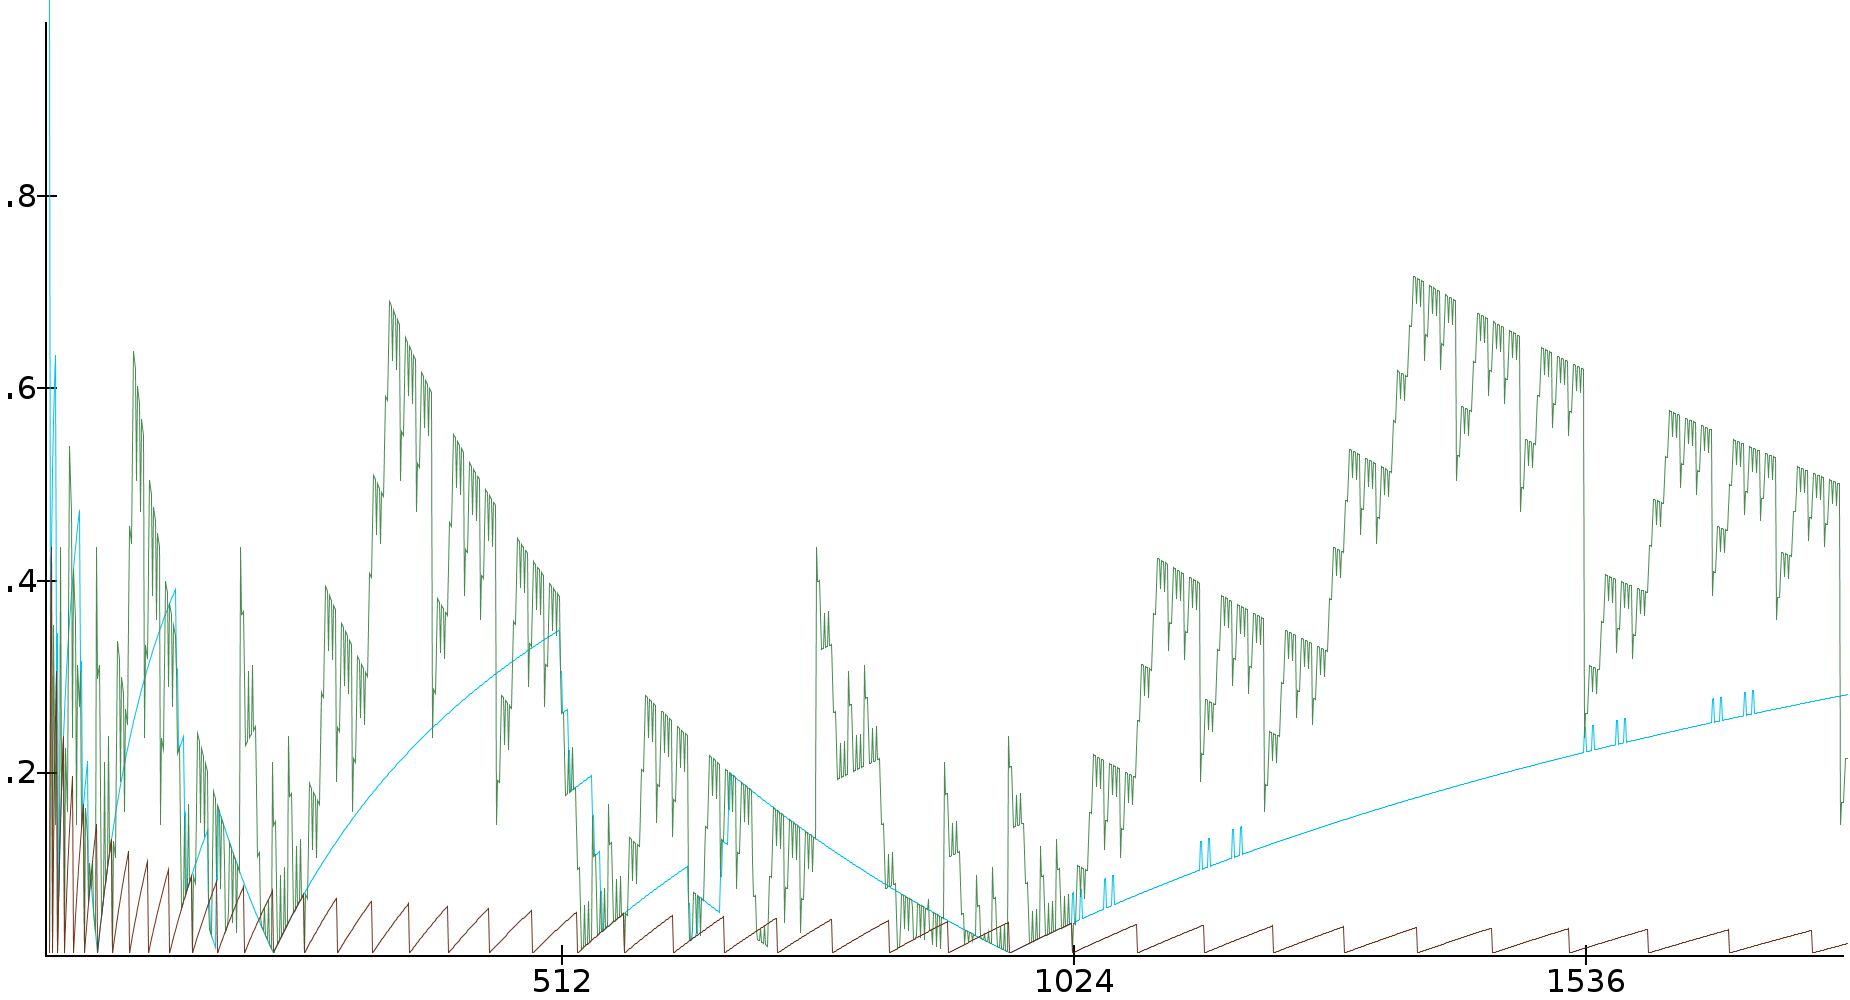
\includegraphics[width=0.75\linewidth]{figure/rel_error_480x.png} 
			\caption{Relative error for the simple square root approximator
				(green), the improved version (blue), and the shifting nth root
				algorithm (red).}
			\label{sres2}
		\end{figure}

		\begin{figure}[H]
			\centering
			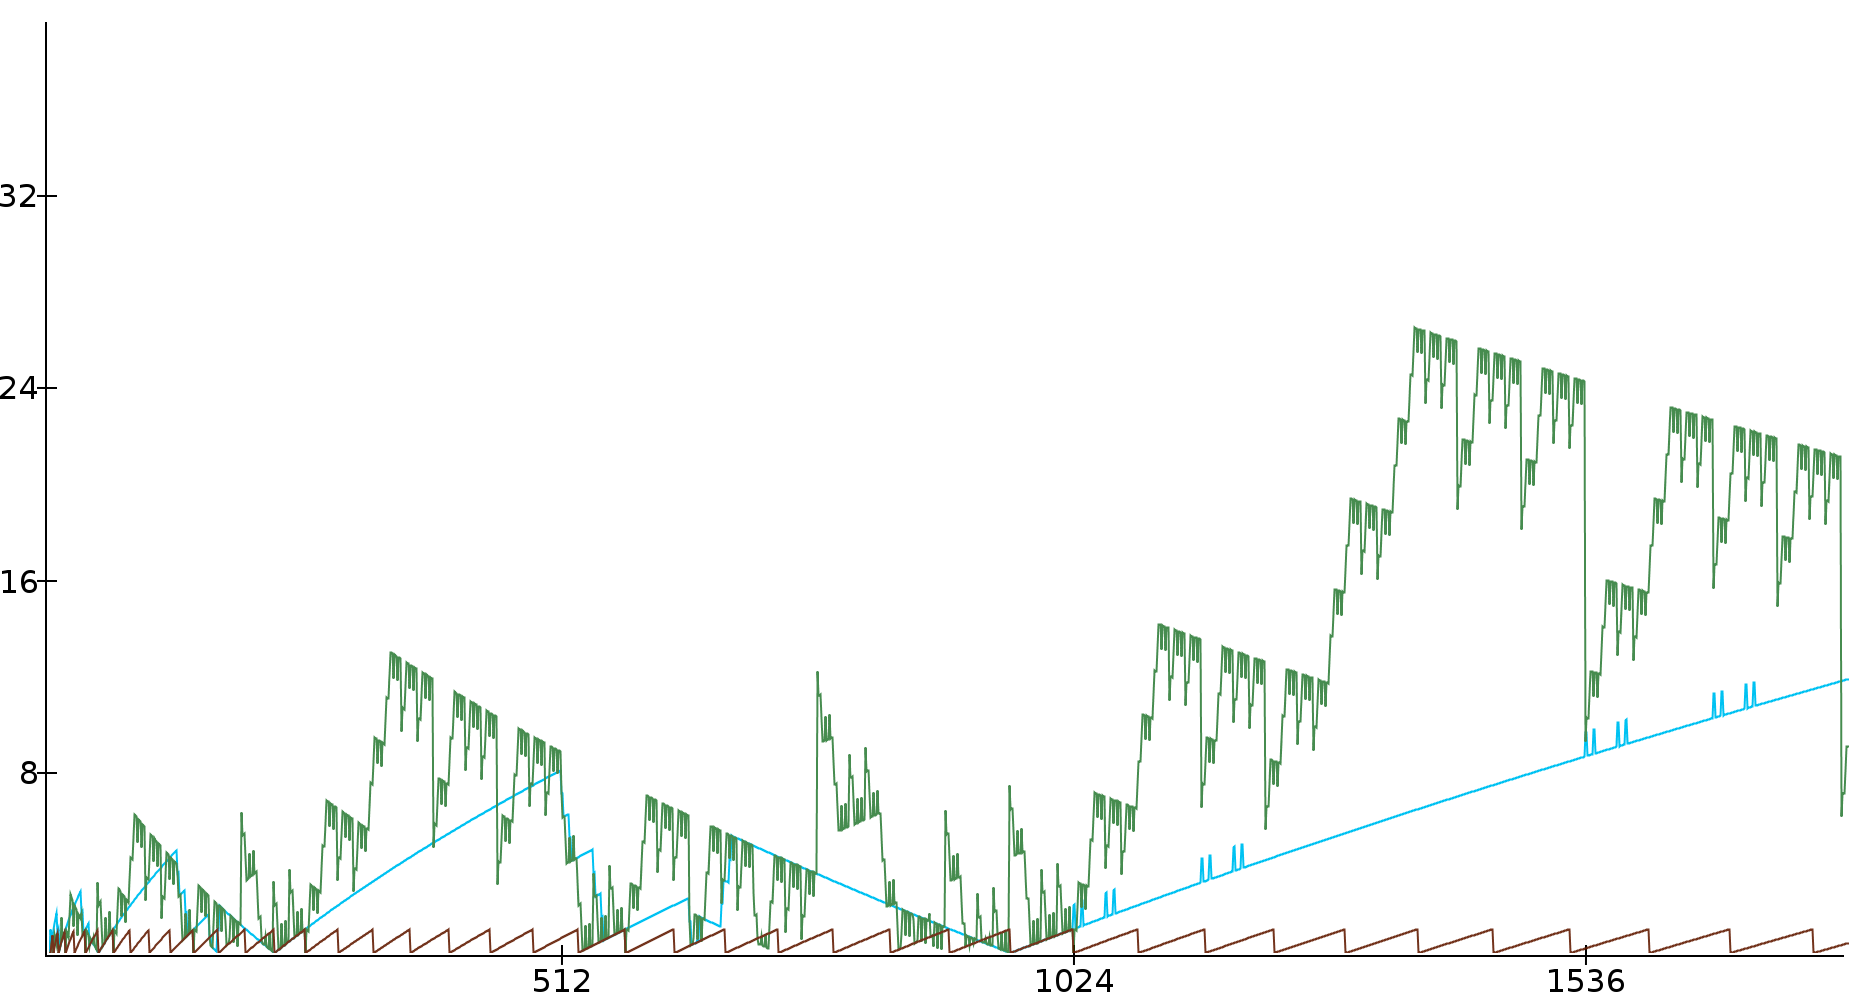
\includegraphics[width=0.75\linewidth]{figure/abs_error_24x.png} 
			\caption{Absolute error for the simple square root approximator
				(green), the improved version (blue), and the shifting nth root
				algorithm (red).}
			\label{sres3}
		\end{figure}

		\begin{figure}[H]
			\centering
			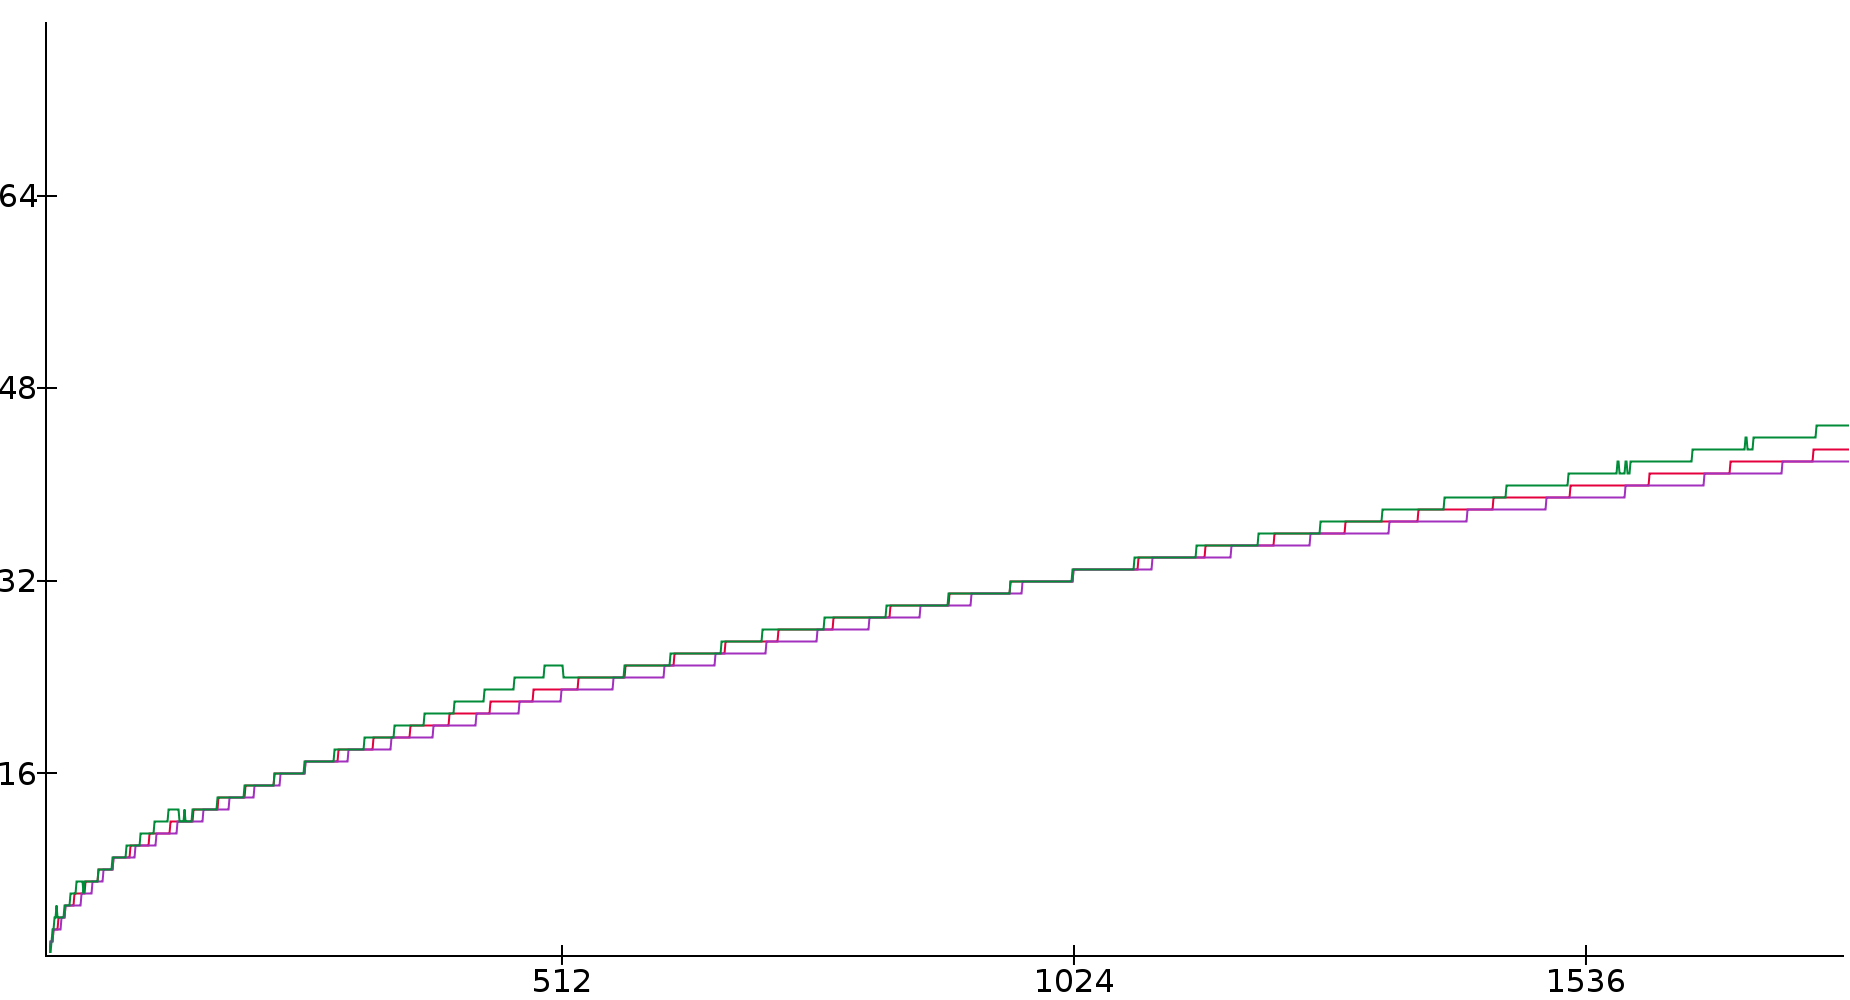
\includegraphics[width=0.75\linewidth]{figure/value_lin12x.png} 
			\caption{Value from lerp-approximator (purple), simple square root
				approximator with one step of the babylonian method (green),
				and the shifting nth root algorithm (red). In these graphs, 
				they all operate on integers. The shifting nth root is exact 
				for integer square roots.}
			\label{sres4}
		\end{figure}

		\begin{figure}[H]
			\centering
			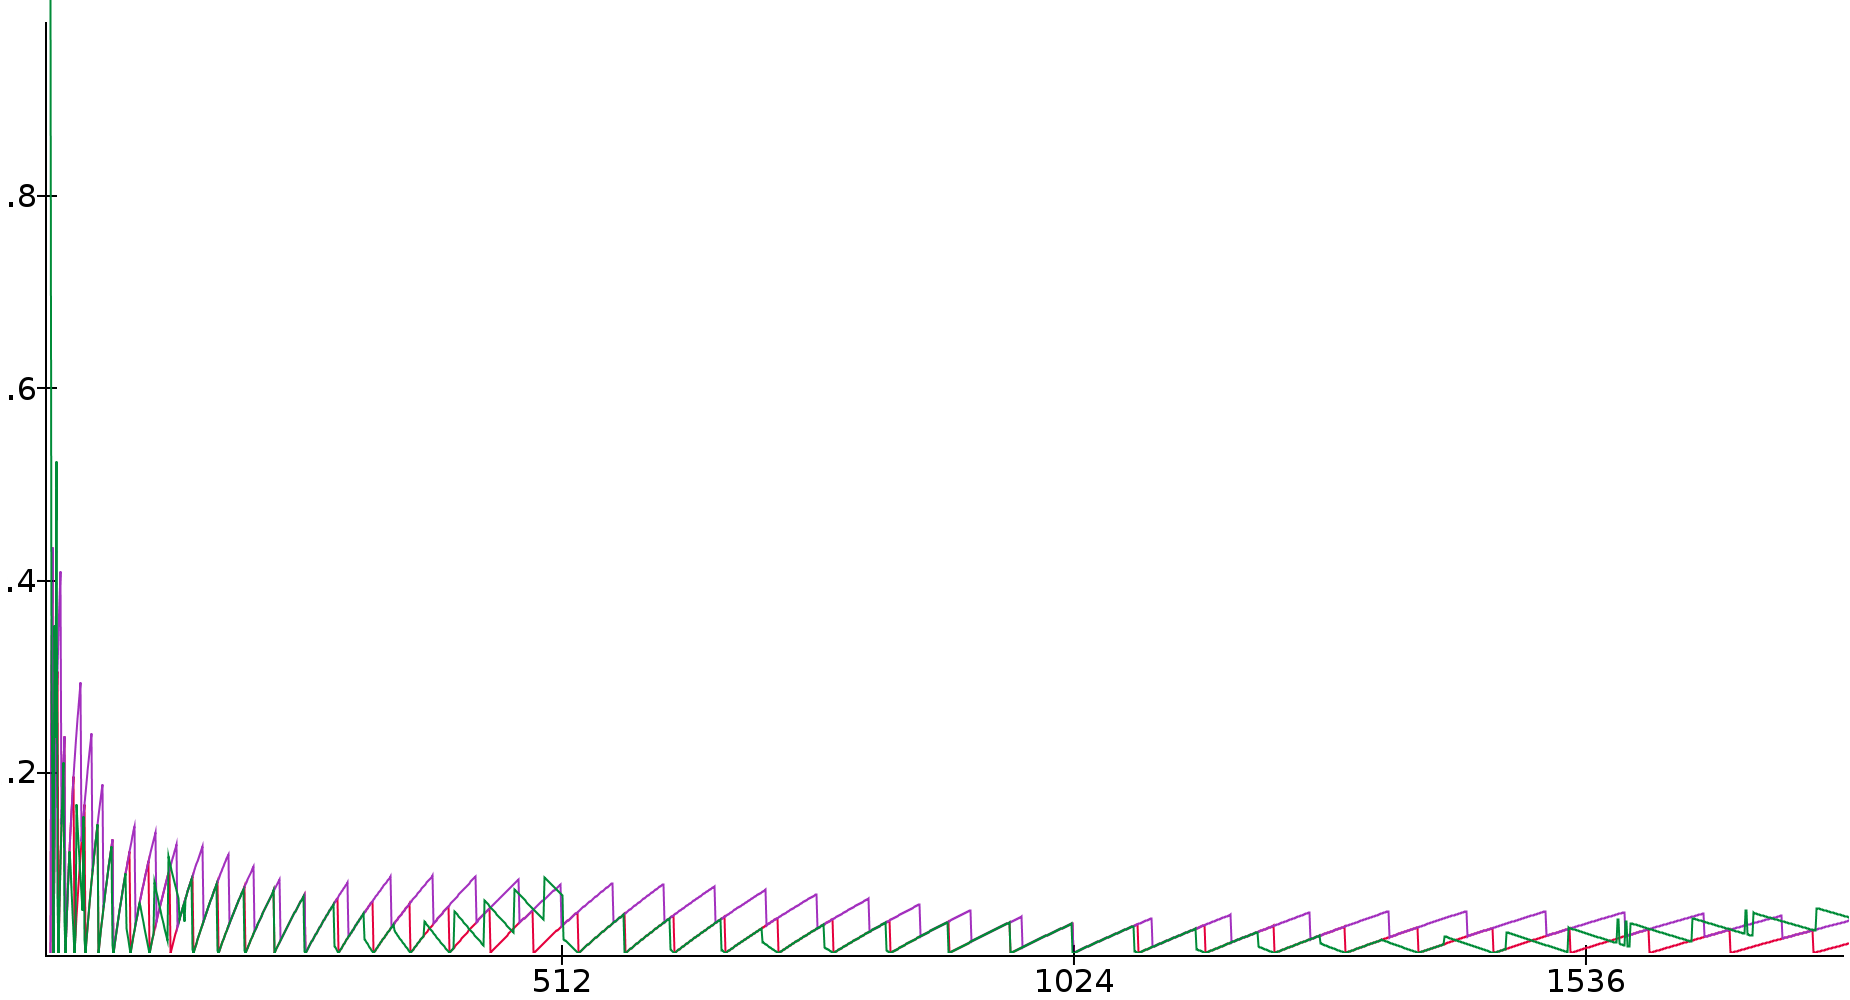
\includegraphics[width=0.75\linewidth]{figure/rel_lin960x.png} 
			\caption{Relative error for the lerp-approximator (purple), simple 
				square root approximator with one step of the babylonian method 
				(green), and the shifting nth root algorithm (red).}
			\label{sres5}
		\end{figure}

		\begin{figure}[H]
			\centering
			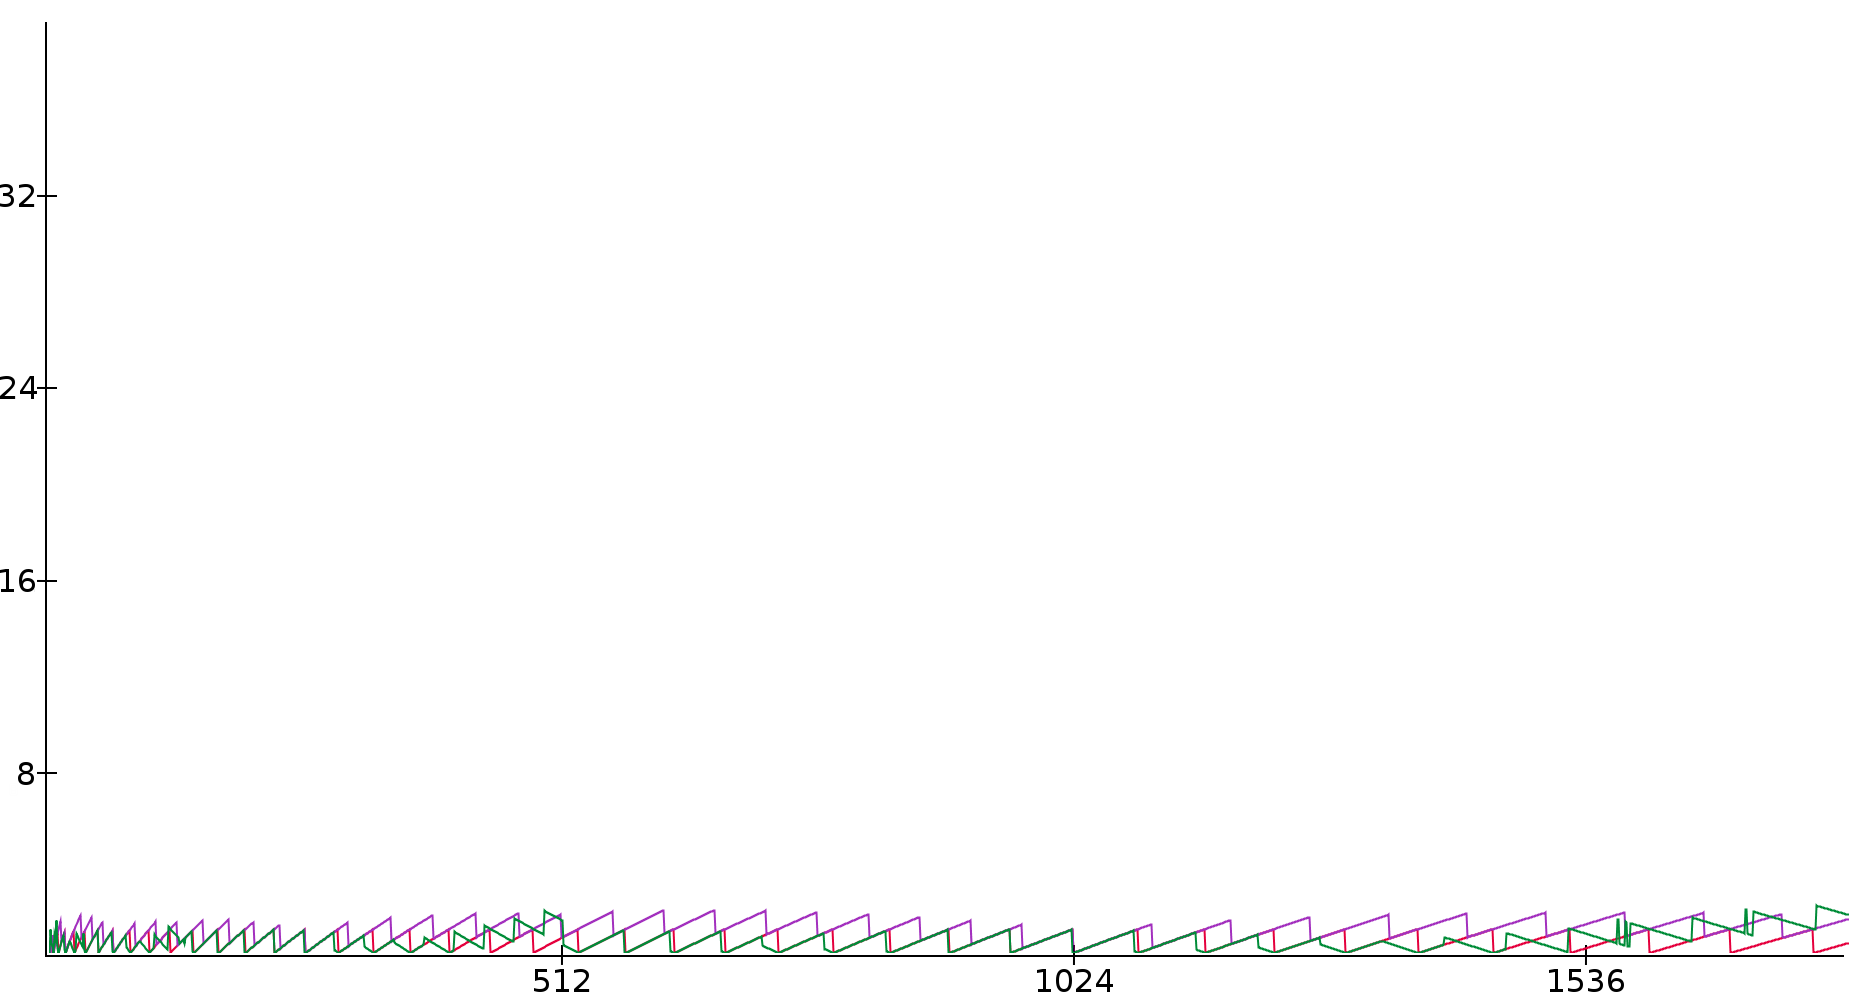
\includegraphics[width=0.75\linewidth]{figure/abs_lin24x.png} 
			\caption{Absolute error for the lerp-approximator (purple), simple 
				square root approximator with one step of the babylonian method 
				(green), and the shifting nth root algorithm (red).}
			\label{sres6}
		\end{figure}

	\section{Optimizations}
		
		During this project, a number of optimizations were discussed and
		developed. Implemented optimizations are explained below and the
		theoretical ones are presented in chapter \ref{discussion} and
		\ref{optimization}. Some of these are based on earlier work, while
		others are believed to be quite unique optimizations which have not been
		discussed for sphere tracing previously. All implemented optimizations
		that affects the algorithm were implemented in the software shader, not
		on our own GPU.

		For all tests performed, FPS (Frames Per Second) is used to measure
		performance. FPS is simply how many times the GPU is able to render 
		the scene per second. The time it takes to render the scene once is 
		equal to one divided by the FPS.

		\subsection{Orthogonal culling}
		
		Tests to see the performance of the orthogonal culling optimization
		were performed by putting an increasing number of solid-colored spheres
		in a plane in front of the camera. Because of this, the spheres are not
		obstructed by other spheres, making this the best possible scenario for
		the optimization.

		Below are test results from Orthogonal culling.

			\begin{table}
			\centering
			\begin{tabular}{lll}
				\hline
				Objects & Optimized & Unoptimized \\ 
				\hline
				1       & 600       & 350         \\ 
				5       & 430       & 180         \\			
				10      & 290       & 98          \\
				15      & 85        & 13          \\
				20      & 58        & 9           \\
				25      & 40        & 6           \\
				30      & 29        & 4           \\
				35      & 7         & 3           \\
				40      & 6         & 2           \\
				45      & 4         & 1.5         \\
				\hline
			\end{tabular}
			\caption{Frames generated per second using the GLSL shader with and
				without the orthogonal culling optimization.}
			\end{table}

			%CHARTS

		\subsection{Bounding spheres}

			Bounding spheres were implemented and tested. There was a clear
			gain in performance in some cases, but the results are very
			situational, depending on too many factors (number of objects, the
			dispersion of objects, size and place of the bounding sphere, etc.)
			to be able to review properly at this time, will be a subject of
			future work. The larger the bounding sphere, the less performance
			gain will be seen and the more objects that can fit into a bounding
			sphere the more performance gain will be seen. 


% DISCUSSION
\chapter{Discussion} 

	This chapter will discuss our thoughts on our result, our theoretical not
	yet	implemented optimizations, and what future work is possible from this
	point in time.
	
	\section{Results}  \label{discussion}
		
		\subsection{Software Shader}

			The optimizations that were implemented improved performance more
			than anticipated. There are many optimizations that are yet to be
			implemented and tested and it's hard to estimate the potential
			achievable performance, the only thing that is certain is that
			there are massive performance potentials.

			There are great limitations in what could be done with the shader
			because of the language that we chose to implement it in, GLSL. It
			offers nothing more than a way to write a program which will run on
			a per-pixel basis and put the result on the screen. Because of
			this, CPU-GPU cooperation is not possible and that comes with
			consequences.

			Modern graphics engines not only does a lot of work on the CPU but
			it has granular control over the GPU, whereas we have no control at

			all. Things such as object positioning, frustum culling, etc.
			should be done by the CPU, not the GPU. This kind of implementation
			can not be done in GLSL and therefore a high-performance sphere
			tracer should be done not in GLSL but in a lower-level language.

			Although GLSL has it's limits it still has some very attractive
			features, it was easy to learn because the syntax has much in
			common with java, which we've studied. The time it takes to develop
			new features and test them is short. The purpose of the software
			shader was to study the algorithm, implement and test optimizations
			and develop new features. For the purposes of this sphere tracer
			GLSL was a perfect fit.
		
		\subsection{GPU} 
		
			The project originally intended to create a simple single-core GPU
			that could fully render a scene given enough time, and then add	
			components as time allowed. As happens with projects like these,
			every design decision one makes clarifies what further needs to be
			done, and reveals previously unseen flaws in the design that must
			be resolved. In the end we implemented the core and a storage 
			manager which enabled multiple cores running in parallel.

			The storage manager turned out to need to be more complex than we 
			originally anticipated. In its first implementation, the storage in
			the storage manager was a simple FIFO queue. This worked well for 
			very simple shader programs, but we found that it was not possible
			to write a full Sphere Tracer using this storage type. This was not
			due to any complexity inherent in the sphere tracing algorithm, but
			rather a consequence of how the GPU requires the shader programs to
			keep track of all pixels they need to render. This is solved by 
			having the shader generate a new thread for every pixel it needs to
			render, and then running the actual pixel shader code on that 
			thread. This fails when threads need to execute many jumps or 
			loops, which are also solved by spawning new threads. Whenever a 
			thread executed a jump, the pixel spawning thread took priority 
			because of the FIFO storage, and a new pixel thread would be 
			spawned. After many jumps, the storage in the storage manager would 
			fill upp entirely, and all cores would stall waiting for the 
			storage manager allowing them to send it more threads. This was 
			solved by changing the internal storage to a double-ended queue,
			giving the threads some control over execution priority.

			If we were to continue working on this project another workflow
			would be adopted when developing the GPU. More detailed planning is
			required in the early stages and empiric testing of different
			implementations is required along the entire development to reach
			the best possible solution.

	\section{Optimizations} \label{optimization}

		\subsection{Bounding spheres}

			Although an increase in performance could be seen using this
			method, it can also be used in ways that decreases the performance.
			By setting up a too large bounding sphere or by setting it up with
			few objects or simply objects that are far apart.

			In testing we saw an increase in performance, but in some cases a
			decrease could also be observed. The performance increase depends
			on a lot of factors such as number of objects in a sphere, how well
			the sphere is fits around them and how far apart they are. If
			misused the performance will be decreased.

			To use this optimization efficiently the objects inside a bounding
			sphere should never come far apart and the sphere should be exactly
			the right size.

		\subsection{Orthogonal culling}

			The performance gain from this optimization exceeded our 
			expectations. This could probably be further improved by 
			implementing the Sphere tracer in a language that has more granular 
			GPU control than GLSL, which is what we used in this paper.

			However great the performance gain the way this is implemented is
			still far from the optimal solution, currently it performs
			orthogonal culling on all the objects in the scene per pixel.
			Instead, culling should be done on a per-object basis and calculate
			which rays an object intersects, this way fewer calculations would
			have to be performed and optimally they would be performed on the
			CPU.

			This method could work together with the Bounding Sphere
			optimization. Instead of projecting single objects onto the ray,
			bounding spheres could be culled, decreasing the number of
			orthogonal projections that has to be made. This too was tested and
			an increase in performance was observed.

	\section{Square roots}

		The simple square root approximator and its improved version are
		extremely simple circuits, indeed they are signifcantly smaller than
		most other common operations performed on numbers in hardware. Of
		course, they are far from accurate, but we find it interesting that it
		is possible to acheive a bounded relative error from the true square
		root for any number of input bits with these small circuits. When
		combined with linear interpolation or iterative methods like the
		Babylonian method the accuracy of these approximations increases
		signifcantly.
		
		The shifting nth root algorithm is the only bit-accurate method tested,
		and it performs well, albeit slower than the approximations. If
		non-exact results are acceptable, which they often are to some extent
		when doing sphere tracing, the number of steps in the shifting nth root
		algorithm could be reduced, which would both increase speed and
		decrease area usage. The lerp-based and iterative methods might still
		be able to reuse common components such as adders and multipliers
		however, and might therefore be preferable.
		
		For the XQBGPPPU, we have used the shifting nth root algorithm in order
		to not have to consider possible accuracy problems when debugging
		shaders, but all methods are implemented and ready to be switched out
		at any time.

	\section{Future work}

		\subsection{GPU-CPU cooperation}

			In the current implementation everything is performed on the GPU,
			including object transformations and culling. Currently if objects
			in the scene are supposed to move they have to be moved using
			mathematical functions, such as sinus. These functions are then
			evaluated for each march step. This is essentially wasted computing
			power and could be performed on the CPU as is standard in modern
			graphics engines.

		\subsection{Plane-ray intersection}

			Infinite planes currently require a lot of computing power to
			render. When the camera is oriented so that the field of view is
			along an infinite plane some rays will travel parallel to the
			plane. These rays will march equally long steps until their max
			number of steps has been taken or the max range has been reached, 
			without hitting anything. This will cause some rays to draw 
			computing power without ever being able to hit the plane anyway. 
			Some rays that should hit the plane will fail to do so because of 
			to many steps taken, making it look like the plane has an edge 
			because after a certain range it is no longer being rendered.

			One potential problem is that because no distance field evaluations 
			are performed, it might be hard to perform Boolean operations or 
			mathematical deformations on planes rendered this way. Another is 
			that every time we add more features that aren't part of the 
			regular Sphere Tracing, the complexity of the program increases. 
			Thus, the advantages of the individual optimizations must be 
			weighed against the overall performance loss they incur. 

		\subsection{Overstepping}

			Bounding spheres technique is somewhat similar to the normal sphere
			tracing. The difference is that when you march you march to the
			edge of the MDS and then you march to the next MDS edge. With
			overstepping technique you march a small distance further outside
			the MDS edge. You then compare the original MDS with the new MDS if
			these two spheres overlap in any way we can march that little bit
			further. By marching that little bit further, decrease in the
			number of times marched is achieved. Giving an increase in
			performance. 

		\subsection{Ray grouping}
		
			Ray grouping works by grouping adjacent rays together. If a
			specific pixel N is to be rendered we group the adjacent pixels
			into a set, then march along the ray of N. If any of the pixels are
			not inside the minimum distance spheres (MDS) the combined pixel is
			split up into smaller sets, which each have a centered pixel. Each
			set then repeats the these steps over and over again individually
			along their new center pixel's ray.  This is repeated a number of
			times depending on the march distance in the scene for every set.
			The closer the sets are to a target, the more likely it is for a
			higher amount of subsets to be created due to the decrease of the
			MDS's volumes making less pixels fit inside.
			
			We believe ray grouping gives a performance increase by lowering
			the number of steps needed to march. Depending on the scene it
			could lower the steps significantly. One example would be a scene
			with only one object in it let's say a sphere, this implies that
			the MDS's volume will be substantial. This will in turn make the
			number of subgroups very low and give us a a performance gain. 
			
			A very complex scene with many objects creates very varying MDS
			volumes which would not give as good of a result as the earlier
			mentioned example due to the increase in subsets early in the
			marching.

	\section{Societal implications}

		There will be no big inpact on society from the results described in
		this report as it stands right now. The GPU is still too underdeveloped
		to definively show if the algorithm has potential one way or another.
		Further prototypes needs to be built with greater rigor before that can
		happen.  If we however assume that somewhere down the line it turns out
		to be a success, then there are generally three ways in which we could
		forsee that happening.

		First up is by breaking through in the games industry. Granted that it
		probably will not be able to outperform modern graphic cards at their
		own game, but the up-and-coming VR technology faces different
		challenges, usually rendering smaller scenes with fewer objects and
		capturing actual ``3D’’ images to display to the user. Both of these
		factors favors Sphere Tracing since it inherently produces perfect 3D
		objects and works much faster in scenes with shorter render distance.

		Another possibility is that the GPU turns out to be too slow for
		rendering games in real time, but runs other Ray Tracing algorithms
		commonly used in movie production faster that modern graphic cards.
		This is not too unlikely since the calculation of the rays in both
		cases follow many similar patterns in bouncing and reflecting etc.
		Since movies render in render farms where like server farms, lots of
		copies of the same hardware works in tandem. Meaning that even a small
		improvement over current graphic cards might be amplified to a
		significant gain in computational power.

		Finally, since we wrote the hardware similar to a CPU but with more
		threading like a GPU except with no lockstepping, it might be a perfect
		fit for some problem not yet discovered. Much like GPUs used to sit
		unused while not being used for gaming or video editing essentialy
		wasting potential computations. Novel projects like
		Folding@Home\cite{Beberg2009} popped up to exploit this fact to a great
		success. Although it is hard to guess at exactly how. Given the
		uniqueness of the hardware it might find a similar novel use in the
		future.


% CONCLUSION
% CREATED BY DAVID FRISK, 2016
\chapter{Conclusion}
	\section{How does sphere tracing work?}

	\section{What language is best suited to describe the GPU?}
	
	The two FHDLs, lava2000 and \clash, not being fully developed languages both produced obtuse and redundant code and in the case of \clash even unsynthezisable code (bug). In the end we decided to go with \clash and it did allow us to type less and to have a more clear overview of the GPU and its components.

	\section{Are there ways we can improve the algorithm at a theoretical level?}



	\section{How do we architect for parrallelism and multiple cores?}

	\section{How do we handle cache in a smart way?}

	\section{What mathematical functions are best implemented in hardware vs software regarding?}

% REFERENCES / BIBLIOGRAPHY
\cleardoublepage
\addcontentsline{toc}{chapter}{Bibliography}
% CREATED BY DAVID FRISK, 2016

\nocite{*}
\bibliographystyle{abbrvurl}
\bibliography{DATX02-17-12}


% APPENDICES
\cleardoublepage
\appendix
\setcounter{page}{1}
\pagenumbering{Roman}

% CREATED BY DAVID FRISK, 2016
\chapter{XQBGPPPU Instruction Listing}

\chapter{XQBGPPPU Assembly}


\end{document}
